\documentclass[12pt]{article}

%packages
%\usepackage{latexsym}
\usepackage{graphicx}
\usepackage{wrapfig}
\usepackage{color}
\usepackage{amsmath}
\usepackage{dsfont}
\usepackage{placeins}
\usepackage{amssymb}
\usepackage{skull}
\usepackage{enumerate}
\usepackage{soul}
\usepackage{alphalph}
\usepackage{hyperref}
\usepackage{enumerate}
\usepackage{listings}
\usepackage{multicol}
\usepackage{etoolbox}
%\usepackage{fancyhdr}

%\fancyhf{} % clear all header and footers
%\renewcommand{\headrulewidth}{0pt} % remove the header rule
%\fancyfoot[LE, LO]{\thepage}


%\usepackage{pstricks,pst-node,pst-tree}

%\usepackage{algpseudocode}
%\usepackage{amsthm}
%\usepackage{hyperref}
%\usepackage{mathrsfs}
%\usepackage{amsfonts}
%\usepackage{bbding}
%\usepackage{listings}
%\usepackage{appendix}
\usepackage[margin=1in]{geometry}
%\geometry{papersize={8.5in,11in},total={6.5in,9in}}
\usepackage{cancel}
%\usepackage{algorithmic, algorithm}

\definecolor{dkgreen}{rgb}{0,0.6,0}
\definecolor{gray}{rgb}{0.5,0.5,0.5}
\definecolor{mauve}{rgb}{0.58,0,0.82}
\lstset{ %
  language=R,                     % the language of the code
  basicstyle=\footnotesize,       % the size of the fonts that are used for the code
  numbers=left,                   % where to put the line-numbers
  numberstyle=\tiny\color{gray},  % the style that is used for the line-numbers
  stepnumber=1,                   % the step between two line-numbers. If it's 1, each line
                                  % will be numbered
  numbersep=5pt,                  % how far the line-numbers are from the code
  backgroundcolor=\color{white},  % choose the background color. You must add \usepackage{color}
  showspaces=false,               % show spaces adding particular underscores
  showstringspaces=false,         % underline spaces within strings
  showtabs=false,                 % show tabs within strings adding particular underscores
  frame=single,                   % adds a frame around the code
  rulecolor=\color{black},        % if not set, the frame-color may be changed on line-breaks within not-black text (e.g. commens (green here))
  tabsize=2,                      % sets default tabsize to 2 spaces
  captionpos=b,                   % sets the caption-position to bottom
  breaklines=true,                % sets automatic line breaking
  breakatwhitespace=false,        % sets if automatic breaks should only happen at whitespace
  title=\lstname,                 % show the filename of files included with \lstinputlisting;
                                  % also try caption instead of title
  keywordstyle=\color{black},      % keyword style
  commentstyle=\color{dkgreen},   % comment style
  stringstyle=\color{mauve},      % string literal style
  escapeinside={\%*}{*)},         % if you want to add a comment within your code
  morekeywords={*,...}            % if you want to add more keywords to the set
}

\newcommand{\qu}[1]{``#1''}
\newcommand{\spc}[1]{\\ \vspace{#1cm}}

\newcounter{probnum}
\setcounter{probnum}{1}

%create definition to allow local margin changes
\def\changemargin#1#2{\list{}{\rightmargin#2\leftmargin#1}\item[]}
\let\endchangemargin=\endlist 

%allow equations to span multiple pages
\allowdisplaybreaks

%define colors and color typesetting conveniences
\definecolor{gray}{rgb}{0.5,0.5,0.5}
\definecolor{black}{rgb}{0,0,0}
\definecolor{white}{rgb}{1,1,1}
\definecolor{blue}{rgb}{0.5,0.5,1}
\newcommand{\inblue}[1]{\color{blue}#1 \color{black}}
\definecolor{green}{rgb}{0.133,0.545,0.133}
\newcommand{\ingreen}[1]{\color{green}#1 \color{black}}
\definecolor{yellow}{rgb}{1,0.549,0}
\newcommand{\inyellow}[1]{\color{yellow}#1 \color{black}}
\definecolor{red}{rgb}{1,0.133,0.133}
\newcommand{\inred}[1]{\color{red}#1 \color{black}}
\definecolor{purple}{rgb}{0.58,0,0.827}
\newcommand{\inpurple}[1]{\color{purple}#1 \color{black}}
\definecolor{gray}{rgb}{0.5,0.5,0.5}
\newcommand{\ingray}[1]{\color{gray}#1 \color{black}}
\definecolor{backgcode}{rgb}{0.97,0.97,0.8}
\definecolor{Brown}{cmyk}{0,0.81,1,0.60}
\definecolor{OliveGreen}{cmyk}{0.64,0,0.95,0.40}
\definecolor{CadetBlue}{cmyk}{0.62,0.57,0.23,0}

%define new math operators
\DeclareMathOperator*{\argmax}{arg\,max~}
\DeclareMathOperator*{\argmin}{arg\,min~}
\DeclareMathOperator*{\argsup}{arg\,sup~}
\DeclareMathOperator*{\arginf}{arg\,inf~}
\DeclareMathOperator*{\convolution}{\text{\Huge{$\ast$}}}
\newcommand{\infconv}[2]{\convolution^\infty_{#1 = 1} #2}
%true functions

%%%% GENERAL SHORTCUTS

\makeatletter
\newalphalph{\alphmult}[mult]{\@alph}{26}
\renewcommand{\labelenumi}{(\alphmult{\value{enumi}})}
\renewcommand{\theenumi}{\AlphAlph{\value{enumi}}}
\makeatother
%shortcuts for pure typesetting conveniences
\newcommand{\bv}[1]{\boldsymbol{#1}}

%shortcuts for compound constants
\newcommand{\BetaDistrConst}{\dfrac{\Gamma(\alpha + \beta)}{\Gamma(\alpha)\Gamma(\beta)}}
\newcommand{\NormDistrConst}{\dfrac{1}{\sqrt{2\pi\sigma^2}}}

%shortcuts for conventional symbols
\newcommand{\tsq}{\tau^2}
\newcommand{\tsqh}{\hat{\tau}^2}
\newcommand{\sigsq}{\sigma^2}
\newcommand{\sigsqsq}{\parens{\sigma^2}^2}
\newcommand{\sigsqovern}{\dfrac{\sigsq}{n}}
\newcommand{\tausq}{\tau^2}
\newcommand{\tausqalpha}{\tau^2_\alpha}
\newcommand{\tausqbeta}{\tau^2_\beta}
\newcommand{\tausqsigma}{\tau^2_\sigma}
\newcommand{\betasq}{\beta^2}
\newcommand{\sigsqvec}{\bv{\sigma}^2}
\newcommand{\sigsqhat}{\hat{\sigma}^2}
\newcommand{\sigsqhatmlebayes}{\sigsqhat_{\text{Bayes, MLE}}}
\newcommand{\sigsqhatmle}[1]{\sigsqhat_{#1, \text{MLE}}}
\newcommand{\bSigma}{\bv{\Sigma}}
\newcommand{\bSigmainv}{\bSigma^{-1}}
\newcommand{\thetavec}{\bv{\theta}}
\newcommand{\thetahat}{\hat{\theta}}
\newcommand{\thetahatmm}{\hat{\theta}^{\mathrm{MM}}}
\newcommand{\thetahathatmm}{\thetahathat^{\mathrm{MM}}}
\newcommand{\thetahathatmle}{\thetahathat^{\mathrm{MLE}}}
\newcommand{\thetahatmle}{\hat{\theta}^{\mathrm{MLE}}}
\newcommand{\thetavechatmle}{\hat{\thetavec}^{\mathrm{MLE}}}
\newcommand{\muhat}{\hat{\mu}}
\newcommand{\muhathat}{\doublehat{\mu}}
\newcommand{\musq}{\mu^2}
\newcommand{\muvec}{\bv{\mu}}
\newcommand{\muhatmle}{\muhat_{\text{MLE}}}
\newcommand{\lambdahat}{\hat{\lambda}}
\newcommand{\lambdahatmle}{\lambdahat_{\text{MLE}}}
\newcommand{\thetahatmap}{\hat{\theta}_{\mathrm{MAP}}}
\newcommand{\thetahatmmae}{\hat{\theta}_{\mathrm{MMAE}}}
\newcommand{\thetahatmmse}{\hat{\theta}_{\mathrm{MMSE}}}
\newcommand{\etavec}{\bv{\eta}}
\newcommand{\alphavec}{\bv{\alpha}}
\newcommand{\minimaxdec}{\delta^*_{\mathrm{mm}}}
\newcommand{\ybar}{\bar{y}}
\newcommand{\xbar}{\bar{x}}
\newcommand{\Xbar}{\bar{X}}
\newcommand{\iid}{~{\buildrel iid \over \sim}~}
\newcommand{\inddist}{~{\buildrel ind \over \sim}~}
\newcommand{\approxdist}{~{\buildrel \bv{\cdot} \over \sim}~}
\newcommand{\equalsindist}{~{\buildrel d \over =}~}
\newcommand{\loglik}[1]{\ell\parens{#1}}
\newcommand{\thetahatkminone}{\thetahat^{(k-1)}}
\newcommand{\thetahatkplusone}{\thetahat^{(k+1)}}
\newcommand{\thetahatk}{\thetahat^{(k)}}
\newcommand{\half}{\frac{1}{2}}
\newcommand{\third}{\frac{1}{3}}
\newcommand{\twothirds}{\frac{2}{3}}
\newcommand{\fourth}{\frac{1}{4}}
\newcommand{\fifth}{\frac{1}{5}}
\newcommand{\sixth}{\frac{1}{6}}

%shortcuts for vector and matrix notation
\newcommand{\A}{\bv{A}}
\newcommand{\At}{\A^T}
\newcommand{\Ainv}{\inverse{\A}}
\newcommand{\B}{\bv{B}}
\renewcommand{\b}{\bv{b}}
\renewcommand{\H}{\bv{H}}
\newcommand{\K}{\bv{K}}
\newcommand{\Kt}{\K^T}
\newcommand{\Kinv}{\inverse{K}}
\newcommand{\Kinvt}{(\Kinv)^T}
\newcommand{\M}{\bv{M}}
\newcommand{\Bt}{\B^T}
\newcommand{\Q}{\bv{Q}}
\newcommand{\Qt}{\Q^T}
\newcommand{\R}{\bv{R}}
\newcommand{\Rt}{\R^T}
\newcommand{\Z}{\bv{Z}}
\newcommand{\X}{\bv{X}}
\newcommand{\Xsub}{\X_{\text{(sub)}}}
\newcommand{\Xsubadj}{\X_{\text{(sub,adj)}}}
\newcommand{\I}{\bv{I}}
\newcommand{\Y}{\bv{Y}}
\newcommand{\sigsqI}{\sigsq\I}
\renewcommand{\P}{\bv{P}}
\newcommand{\Psub}{\P_{\text{(sub)}}}
\newcommand{\Pt}{\P^T}
\newcommand{\Pii}{P_{ii}}
\newcommand{\Pij}{P_{ij}}
\newcommand{\IminP}{(\I-\P)}
\newcommand{\Xt}{\bv{X}^T}
\newcommand{\XtX}{\Xt\X}
\newcommand{\XtXinv}{\parens{\Xt\X}^{-1}}
\newcommand{\XtXinvXt}{\XtXinv\Xt}
\newcommand{\XXtXinvXt}{\X\XtXinvXt}
\newcommand{\x}{\bv{x}}
\newcommand{\w}{\bv{w}}
\newcommand{\q}{\bv{q}}
\newcommand{\zerovec}{\bv{0}}
\newcommand{\onevec}{\bv{1}}
\newcommand{\oneton}{1, \ldots, n}
\newcommand{\yoneton}{y_1, \ldots, y_n}
\newcommand{\yonetonorder}{y_{(1)}, \ldots, y_{(n)}}
\newcommand{\Yoneton}{Y_1, \ldots, Y_n}
\newcommand{\iinoneton}{i \in \braces{\oneton}}
\newcommand{\onetom}{1, \ldots, m}
\newcommand{\jinonetom}{j \in \braces{\onetom}}
\newcommand{\xoneton}{x_1, \ldots, x_n}
\newcommand{\Xoneton}{X_1, \ldots, X_n}
\newcommand{\xt}{\x^T}
\newcommand{\y}{\bv{y}}
\newcommand{\yt}{\y^T}
\renewcommand{\c}{\bv{c}}
\newcommand{\ct}{\c^T}
\newcommand{\tstar}{\bv{t}^*}
\renewcommand{\u}{\bv{u}}
\renewcommand{\v}{\bv{v}}
\renewcommand{\a}{\bv{a}}
\newcommand{\s}{\bv{s}}
\newcommand{\yadj}{\y_{\text{(adj)}}}
\newcommand{\xjadj}{\x_{j\text{(adj)}}}
\newcommand{\xjadjM}{\x_{j \perp M}}
\newcommand{\yhat}{\hat{\y}}
\newcommand{\yhatsub}{\yhat_{\text{(sub)}}}
\newcommand{\yhatstar}{\yhat^*}
\newcommand{\yhatstarnew}{\yhatstar_{\text{new}}}
\newcommand{\z}{\bv{z}}
\newcommand{\zt}{\z^T}
\newcommand{\bb}{\bv{b}}
\newcommand{\bbt}{\bb^T}
\newcommand{\bbeta}{\bv{\beta}}
\newcommand{\beps}{\bv{\epsilon}}
\newcommand{\bepst}{\beps^T}
\newcommand{\e}{\bv{e}}
\newcommand{\Mofy}{\M(\y)}
\newcommand{\KofAlpha}{K(\alpha)}
\newcommand{\ellset}{\mathcal{L}}
\newcommand{\oneminalph}{1-\alpha}
\newcommand{\SSE}{\text{SSE}}
\newcommand{\SSEsub}{\text{SSE}_{\text{(sub)}}}
\newcommand{\MSE}{\text{MSE}}
\newcommand{\RMSE}{\text{RMSE}}
\newcommand{\SSR}{\text{SSR}}
\newcommand{\SST}{\text{SST}}
\newcommand{\JSest}{\delta_{\text{JS}}(\x)}
\newcommand{\Bayesest}{\delta_{\text{Bayes}}(\x)}
\newcommand{\EmpBayesest}{\delta_{\text{EmpBayes}}(\x)}
\newcommand{\BLUPest}{\delta_{\text{BLUP}}}
\newcommand{\MLEest}[1]{\hat{#1}_{\text{MLE}}}

%shortcuts for Linear Algebra stuff (i.e. vectors and matrices)
\newcommand{\twovec}[2]{\bracks{\begin{array}{c} #1 \\ #2 \end{array}}}
\newcommand{\threevec}[3]{\bracks{\begin{array}{c} #1 \\ #2 \\ #3 \end{array}}}
\newcommand{\fivevec}[5]{\bracks{\begin{array}{c} #1 \\ #2 \\ #3 \\ #4 \\ #5 \end{array}}}
\newcommand{\twobytwomat}[4]{\bracks{\begin{array}{cc} #1 & #2 \\ #3 & #4 \end{array}}}
\newcommand{\threebytwomat}[6]{\bracks{\begin{array}{cc} #1 & #2 \\ #3 & #4 \\ #5 & #6 \end{array}}}

%shortcuts for conventional compound symbols
\newcommand{\thetainthetas}{\theta \in \Theta}
\newcommand{\reals}{\mathbb{R}}
\newcommand{\complexes}{\mathbb{C}}
\newcommand{\rationals}{\mathbb{Q}}
\newcommand{\integers}{\mathbb{Z}}
\newcommand{\naturals}{\mathbb{N}}
\newcommand{\forallninN}{~~\forall n \in \naturals}
\newcommand{\forallxinN}[1]{~~\forall #1 \in \reals}
\newcommand{\matrixdims}[2]{\in \reals^{\,#1 \times #2}}
\newcommand{\inRn}[1]{\in \reals^{\,#1}}
\newcommand{\mathimplies}{\quad\Rightarrow\quad}
\newcommand{\mathlogicequiv}{\quad\Leftrightarrow\quad}
\newcommand{\eqncomment}[1]{\quad \text{(#1)}}
\newcommand{\limitn}{\lim_{n \rightarrow \infty}}
\newcommand{\limitN}{\lim_{N \rightarrow \infty}}
\newcommand{\limitd}{\lim_{d \rightarrow \infty}}
\newcommand{\limitt}{\lim_{t \rightarrow \infty}}
\newcommand{\limitsupn}{\limsup_{n \rightarrow \infty}~}
\newcommand{\limitinfn}{\liminf_{n \rightarrow \infty}~}
\newcommand{\limitk}{\lim_{k \rightarrow \infty}}
\newcommand{\limsupn}{\limsup_{n \rightarrow \infty}}
\newcommand{\limsupk}{\limsup_{k \rightarrow \infty}}
\newcommand{\floor}[1]{\left\lfloor #1 \right\rfloor}
\newcommand{\ceil}[1]{\left\lceil #1 \right\rceil}

%shortcuts for environments
\newcommand{\beqn}{\vspace{-0.25cm}\begin{eqnarray*}}
\newcommand{\eeqn}{\end{eqnarray*}}
\newcommand{\bneqn}{\vspace{-0.25cm}\begin{eqnarray}}
\newcommand{\eneqn}{\end{eqnarray}}
\newcommand{\benum}{\begin{itemize}}
\newcommand{\eenum}{\end{itemize}}

%shortcuts for mini environments
\newcommand{\parens}[1]{\left(#1\right)}
\newcommand{\squared}[1]{\parens{#1}^2}
\newcommand{\tothepow}[2]{\parens{#1}^{#2}}
\newcommand{\prob}[1]{\mathbb{P}\parens{#1}}
\newcommand{\littleo}[1]{o\parens{#1}}
\newcommand{\bigo}[1]{O\parens{#1}}
\newcommand{\Lp}[1]{\mathbb{L}^{#1}}
\renewcommand{\arcsin}[1]{\text{arcsin}\parens{#1}}
\newcommand{\prodonen}[2]{\bracks{\prod_{#1=1}^n #2}}
\newcommand{\mysum}[4]{\sum_{#1=#2}^{#3} #4}
\newcommand{\sumonen}[2]{\sum_{#1=1}^n #2}
\newcommand{\infsum}[2]{\sum_{#1=1}^\infty #2}
\newcommand{\infprod}[2]{\prod_{#1=1}^\infty #2}
\newcommand{\infunion}[2]{\bigcup_{#1=1}^\infty #2}
\newcommand{\infinter}[2]{\bigcap_{#1=1}^\infty #2}
\newcommand{\infintegral}[2]{\int^\infty_{-\infty} #2 ~\text{d}#1}
\newcommand{\supthetas}[1]{\sup_{\thetainthetas}\braces{#1}}
\newcommand{\bracks}[1]{\left[#1\right]}
\newcommand{\braces}[1]{\left\{#1\right\}}
\newcommand{\angbraces}[1]{\left<#1\right>}
\newcommand{\set}[1]{\left\{#1\right\}}
\newcommand{\abss}[1]{\left|#1\right|}
\newcommand{\norm}[1]{\left|\left|#1\right|\right|}
\newcommand{\normsq}[1]{\norm{#1}^2}
\newcommand{\inverse}[1]{\parens{#1}^{-1}}
\newcommand{\rowof}[2]{\parens{#1}_{#2\cdot}}

%shortcuts for functionals
\newcommand{\realcomp}[1]{\text{Re}\bracks{#1}}
\newcommand{\imagcomp}[1]{\text{Im}\bracks{#1}}
\newcommand{\range}[1]{\text{range}\bracks{#1}}
\newcommand{\colsp}[1]{\text{colsp}\bracks{#1}}
\newcommand{\rowsp}[1]{\text{rowsp}\bracks{#1}}
\newcommand{\tr}[1]{\text{tr}\bracks{#1}}
\newcommand{\rank}[1]{\text{rank}\bracks{#1}}
\newcommand{\proj}[2]{\text{Proj}_{#1}\bracks{#2}}
\newcommand{\projcolspX}[1]{\text{Proj}_{\colsp{\X}}\bracks{#1}}
\newcommand{\median}[1]{\text{median}\bracks{#1}}
\newcommand{\mean}[1]{\text{mean}\bracks{#1}}
\newcommand{\dime}[1]{\text{dim}\bracks{#1}}
\renewcommand{\det}[1]{\text{det}\bracks{#1}}
\newcommand{\expe}[1]{\mathbb{E}\bracks{#1}}
\newcommand{\expeabs}[1]{\expe{\abss{#1}}}
\newcommand{\expesub}[2]{\mathbb{E}_{#1}\bracks{#2}}
\newcommand{\cexpesub}[3]{\mathbb{E}_{#1}\bracks{#2~|~#3}}
\newcommand{\indic}[1]{\mathds{1}_{#1}}
\newcommand{\var}[1]{\mathbb{V}\text{ar}\bracks{#1}}
\newcommand{\mse}[1]{\mathbb{M}\text{SE}\bracks{#1}}
\newcommand{\sd}[1]{\mathbb{S}\text{D}\bracks{#1}}
\newcommand{\support}[1]{\mathbb{S}_{#1}}
\newcommand{\cov}[2]{\mathbb{C}\text{ov}\bracks{#1, #2}}
\newcommand{\corr}[2]{\mathbb{C}\text{orr}\bracks{#1, #2}}
\newcommand{\se}[1]{\text{SE}\bracks{#1}}
\newcommand{\seest}[1]{\hat{\text{SE}}\bracks{#1}}
\newcommand{\bias}[1]{\mathbb{B}\text{ias}\bracks{#1}}
\newcommand{\partialop}[2]{\dfrac{\partial}{\partial #1}\bracks{#2}}
\newcommand{\secpartialop}[2]{\dfrac{\partial^2}{\partial #1^2}\bracks{#2}}
\newcommand{\mixpartialop}[3]{\dfrac{\partial^2}{\partial #1 \partial #2}\bracks{#3}}

%shortcuts for functions
\renewcommand{\exp}[1]{\mathrm{exp}\parens{#1}}
\renewcommand{\cos}[1]{\text{cos}\parens{#1}}
\renewcommand{\sin}[1]{\text{sin}\parens{#1}}
\newcommand{\sign}[1]{\text{sign}\parens{#1}}
\newcommand{\are}[1]{\mathrm{ARE}\parens{#1}}
\newcommand{\natlog}[1]{\ln\parens{#1}}
\newcommand{\oneover}[1]{\frac{1}{#1}}
\newcommand{\overtwo}[1]{\frac{#1}{2}}
\newcommand{\overn}[1]{\frac{#1}{n}}
\newcommand{\oversqrtn}[1]{\frac{#1}{\sqrt{n}}}
\newcommand{\oneoversqrt}[1]{\oneover{\sqrt{#1}}}
\newcommand{\sqd}[1]{\parens{#1}^2}
\newcommand{\loss}[1]{\ell\parens{\theta, #1}}
\newcommand{\losstwo}[2]{\ell\parens{#1, #2}}
\newcommand{\cf}{\phi(t)}

%English language specific shortcuts
\newcommand{\ie}{\textit{i.e.} }
\newcommand{\AKA}{\textit{AKA} }
\renewcommand{\iff}{\textit{iff}}
\newcommand{\eg}{\textit{e.g.} }
\renewcommand{\st}{\textit{s.t.} }
\newcommand{\wrt}{\textit{w.r.t.} }
\newcommand{\mathst}{~~\text{\st}~~}
\newcommand{\mathand}{~~\text{and}~~}
\newcommand{\ala}{\textit{a la} }
\newcommand{\ppp}{posterior predictive p-value}
\newcommand{\dd}{dataset-to-dataset}

%shortcuts for distribution titles
\newcommand{\logistic}[2]{\mathrm{Logistic}\parens{#1,\,#2}}
\newcommand{\bernoulli}[1]{\mathrm{Bernoulli}\parens{#1}}
\newcommand{\betanot}[2]{\mathrm{Beta}\parens{#1,\,#2}}
\newcommand{\stdbetanot}{\betanot{\alpha}{\beta}}
\newcommand{\multnormnot}[3]{\mathcal{N}_{#1}\parens{#2,\,#3}}
\newcommand{\normnot}[2]{\mathcal{N}\parens{#1,\,#2}}
\newcommand{\classicnormnot}{\normnot{\mu}{\sigsq}}
\newcommand{\stdnormnot}{\normnot{0}{1}}
\newcommand{\uniform}[2]{\mathrm{U}\parens{#1,\,#2}}
\newcommand{\stduniform}{\uniform{0}{1}}
\newcommand{\exponential}[1]{\mathrm{Exp}\parens{#1}}
\newcommand{\geometric}[1]{\mathrm{Geometric}\parens{#1}}
\newcommand{\gammadist}[2]{\mathrm{Gamma}\parens{#1, #2}}
\newcommand{\negbin}[2]{\mathrm{NegBin}\parens{#1, #2}}
\newcommand{\poisson}[1]{\mathrm{Poisson}\parens{#1}}
\newcommand{\binomial}[2]{\mathrm{Binomial}\parens{#1,\,#2}}
\newcommand{\erlang}[2]{\mathrm{Erlang}\parens{#1,\,#2}}
\newcommand{\rayleigh}[1]{\mathrm{Rayleigh}\parens{#1}}
\newcommand{\multinomial}[3]{\mathrm{Multinom}_{#1}\parens{#2,\,#3}}
\newcommand{\gammanot}[2]{\mathrm{Gamma}\parens{#1,\,#2}}
\newcommand{\cauchynot}[2]{\text{Cauchy}\parens{#1,\,#2}}
\newcommand{\invchisqnot}[1]{\text{Inv}\chisq{#1}}
\newcommand{\invscaledchisqnot}[2]{\text{ScaledInv}\ncchisq{#1}{#2}}
\newcommand{\invgammanot}[2]{\text{InvGamma}\parens{#1,\,#2}}
\newcommand{\chisq}[1]{\chi^2_{#1}}
\newcommand{\ncchisq}[2]{\chi^2_{#1}\parens{#2}}
\newcommand{\ncF}[3]{F_{#1,#2}\parens{#3}}

%shortcuts for PDF's of common distributions
\newcommand{\logisticpdf}[3]{\oneover{#3}\dfrac{\exp{-\dfrac{#1 - #2}{#3}}}{\parens{1+\exp{-\dfrac{#1 - #2}{#3}}}^2}}
\newcommand{\betapdf}[3]{\dfrac{\Gamma(#2 + #3)}{\Gamma(#2)\Gamma(#3)}#1^{#2-1} (1-#1)^{#3-1}}
\newcommand{\normpdf}[3]{\frac{1}{\sqrt{2\pi#3}}\exp{-\frac{1}{2#3}(#1 - #2)^2}}
\newcommand{\normpdfvarone}[2]{\dfrac{1}{\sqrt{2\pi}}e^{-\half(#1 - #2)^2}}
\newcommand{\chisqpdf}[2]{\dfrac{1}{2^{#2/2}\Gamma(#2/2)}\; {#1}^{#2/2-1} e^{-#1/2}}
\newcommand{\invchisqpdf}[2]{\dfrac{2^{-\overtwo{#1}}}{\Gamma(#2/2)}\,{#1}^{-\overtwo{#2}-1}  e^{-\oneover{2 #1}}}
\newcommand{\uniformdiscrete}[1]{\mathrm{Uniform}\parens{\braces{#1}}}
\newcommand{\exponentialpdf}[2]{#2\exp{-#2#1}}
\newcommand{\poissonpdf}[2]{\dfrac{e^{-#1} #1^{#2}}{#2!}}
\newcommand{\binomialpdf}[3]{\binom{#2}{#1}#3^{#1}(1-#3)^{#2-#1}}
\newcommand{\rayleighpdf}[2]{\dfrac{#1}{#2^2}\exp{-\dfrac{#1^2}{2 #2^2}}}
\newcommand{\gammapdf}[3]{\dfrac{#3^#2}{\Gamma\parens{#2}}#1^{#2-1}\exp{-#3 #1}}
\newcommand{\cauchypdf}[3]{\oneover{\pi} \dfrac{#3}{\parens{#1-#2}^2 + #3^2}}
\newcommand{\Gammaf}[1]{\Gamma\parens{#1}}

%shortcuts for miscellaneous typesetting conveniences
\newcommand{\notesref}[1]{\marginpar{\color{gray}\tt #1\color{black}}}

%%%% DOMAIN-SPECIFIC SHORTCUTS

%Real analysis related shortcuts
\newcommand{\zeroonecl}{\bracks{0,1}}
\newcommand{\forallepsgrzero}{\forall \epsilon > 0~~}
\newcommand{\lessthaneps}{< \epsilon}
\newcommand{\fraccomp}[1]{\text{frac}\bracks{#1}}

%Bayesian related shortcuts
\newcommand{\yrep}{y^{\text{rep}}}
\newcommand{\yrepisq}{(\yrep_i)^2}
\newcommand{\yrepvec}{\bv{y}^{\text{rep}}}


%Probability shortcuts
\newcommand{\SigField}{\mathcal{F}}
\newcommand{\ProbMap}{\mathcal{P}}
\newcommand{\probtrinity}{\parens{\Omega, \SigField, \ProbMap}}
\newcommand{\convp}{~{\buildrel p \over \rightarrow}~}
\newcommand{\convLp}[1]{~{\buildrel \Lp{#1} \over \rightarrow}~}
\newcommand{\nconvp}{~{\buildrel p \over \nrightarrow}~}
\newcommand{\convae}{~{\buildrel a.e. \over \longrightarrow}~}
\newcommand{\convau}{~{\buildrel a.u. \over \longrightarrow}~}
\newcommand{\nconvau}{~{\buildrel a.u. \over \nrightarrow}~}
\newcommand{\nconvae}{~{\buildrel a.e. \over \nrightarrow}~}
\newcommand{\convd}{~{\buildrel d \over \rightarrow}~}
\newcommand{\nconvd}{~{\buildrel d \over \nrightarrow}~}
\newcommand{\withprob}{~~\text{w.p.}~~}
\newcommand{\io}{~~\text{i.o.}}

\newcommand{\Acl}{\bar{A}}
\newcommand{\ENcl}{\bar{E}_N}
\newcommand{\diam}[1]{\text{diam}\parens{#1}}

\newcommand{\taua}{\tau_a}

\newcommand{\myint}[4]{\int_{#2}^{#3} #4 \,\text{d}#1}
\newcommand{\laplacet}[1]{\mathscr{L}\bracks{#1}}
\newcommand{\laplaceinvt}[1]{\mathscr{L}^{-1}\bracks{#1}}
\renewcommand{\max}[1]{\text{max}\braces{#1}}
\renewcommand{\min}[1]{\text{min}\braces{#1}}

\newcommand{\Vbar}[1]{\bar{V}\parens{#1}}
\newcommand{\expnegrtau}{\exp{-r\tau}}
\newcommand{\cprob}[2]{\prob{#1~|~#2}}
\newcommand{\ck}[2]{k\parens{#1~|~#2}}

%%% problem typesetting
\newcommand{\problem}{\vspace{0.2cm} \noindent {\large{\textsf{Problem \arabic{probnum}~}}} \addtocounter{probnum}{1}}
%\newcommand{\easyproblem}{\ingreen{\noindent \textsf{Problem \arabic{probnum}~}} \addtocounter{probnum}{1}}
%\newcommand{\intermediateproblem}{\noindent \inyellow{\textsf{Problem \arabic{probnum}~}} \addtocounter{probnum}{1}}
%\newcommand{\hardproblem}{\inred{\noindent \textsf{Problem \arabic{probnum}~}} \addtocounter{probnum}{1}}
%\newcommand{\extracreditproblem}{\noindent \inpurple{\textsf{Problem \arabic{probnum}~}} \addtocounter{probnum}{1}}

\newcommand{\easysubproblem}{\ingreen{\item}}
\newcommand{\intermediatesubproblem}{\inyellow{\item}}
\newcommand{\hardsubproblem}{\inred{\item}}
\newcommand{\extracreditsubproblem}{\inpurple{\item}}


\newcounter{numpts}
\setcounter{numpts}{0}


%\newcommand{\subquestionwithpoints}[1]{\addtocounter{numpts}{#1} \item \ingray{[#1 pt]}~~} %  / \arabic{numpts} pts
\newcommand{\subquestionwithpoints}[1]{\addtocounter{numpts}{#1} \item \ingray{[#1 pt / \arabic{numpts} pts]}~~}  
\newcommand{\truefalsesubquestionwithpoints}[1]{\subquestionwithpoints{#1} Record the letter(s) of all the following that are \textbf{true} in general. At least one will be true.}
\newcommand{\multchoicewithpoints}[2]{\subquestionwithpoints{#1} #2}

\newcounter{nummin}
\setcounter{nummin}{0}

\usepackage{accents}
\newlength{\dhatheight}
\newcommand{\doublehat}[1]{%
    \settoheight{\dhatheight}{\ensuremath{\hat{#1}}}%
    \addtolength{\dhatheight}{-0.35ex}%
    \hat{\vphantom{\rule{1pt}{\dhatheight}}%
    \smash{\hat{#1}}}}
\newcommand{\thetahathat}{\doublehat{\theta}}

%\newcommand{\subquestionwithpoints}[1]{\addtocounter{numpts}{#1} \item \ingray{[#1 pt]}~~} %  / \arabic{numpts} pts
\newcommand{\timedsection}[1]{\addtocounter{nummin}{#1}{[#1min] \ingray{(and \arabic{nummin}min will have elapsed)}}}  
%\newcommand{\timedsection}[1]{\addtocounter{nummin}{#1}{[#1 min]}}


\newtoggle{solutions}
%\toggletrue{solutions}

\newcommand{\instr}{\small Your answer will consist of a lowercase string (e.g. \texttt{aebgd}) where the order of the letters does not matter. \normalsize}

\newcommand{\logbaseten}[1]{\text{log$_{10}$}\parens{#1}}

\title{Math 343 / 643 Spring \the\year{} \\ Midterm Examination One}
\author{Professor Adam Kapelner}

\date{February 27, \the\year{}}

\begin{document}
\maketitle

\noindent Full Name \line(1,0){410}

\thispagestyle{empty}

\section*{Code of Academic Integrity}

\footnotesize
Since the college is an academic community, its fundamental purpose is the pursuit of knowledge. Essential to the success of this educational mission is a commitment to the principles of academic integrity. Every member of the college community is responsible for upholding the highest standards of honesty at all times. Students, as members of the community, are also responsible for adhering to the principles and spirit of the following Code of Academic Integrity.

Activities that have the effect or intention of interfering with education, pursuit of knowledge, or fair evaluation of a student's performance are prohibited. Examples of such activities include but are not limited to the following definitions:

\paragraph{Cheating} Using or attempting to use unauthorized assistance, material, or study aids in examinations or other academic work or preventing, or attempting to prevent, another from using authorized assistance, material, or study aids. Example: using an unauthorized cheat sheet in a quiz or exam, altering a graded exam and resubmitting it for a better grade, etc.\\
\\
\noindent I acknowledge and agree to uphold this Code of Academic Integrity. \\~\\

\begin{center}
\line(1,0){350} ~~~ \line(1,0){100}\\
~~~~~~~~~~~~~~~~~~~~~~~~~~~~~~~~~~signature~~~~~~~~~~~~~~~~~~~~~~~~~~~~~~~~~~~~~~~~~~~~~~~~~~~~~~~~~~~~~~ date
\end{center}

\normalsize

\section*{Instructions}
This exam is 75 minutes (variable time per question) and closed-book. You are allowed \textbf{one} page (front and back) of a \qu{cheat sheet}, blank scrap paper (provided by the proctor) and a graphing calculator (which is not your smartphone). Please read the questions carefully. Within each problem, I recommend considering the questions that are easy first and then circling back to evaluate the harder ones. No food is allowed, only drinks. %If the question reads \qu{compute,} this means the solution will be a number otherwise you can leave the answer in \textit{any} widely accepted mathematical notation which could be resolved to an exact or approximate number with the use of a computer. I advise you to skip problems marked \qu{[Extra Credit]} until you have finished the other questions on the exam, then loop back and plug in all the holes. I also advise you to use pencil. The exam is 100 points total plus extra credit. Partial credit will be granted for incomplete answers on most of the questions. \fbox{Box} in your final answers. Good luck!

\pagebreak

\problem We measure the time (in months) between $n=60$ earthquakes. Here is a scatterplot of the raw data:

\begin{figure}[h]
    \centering
    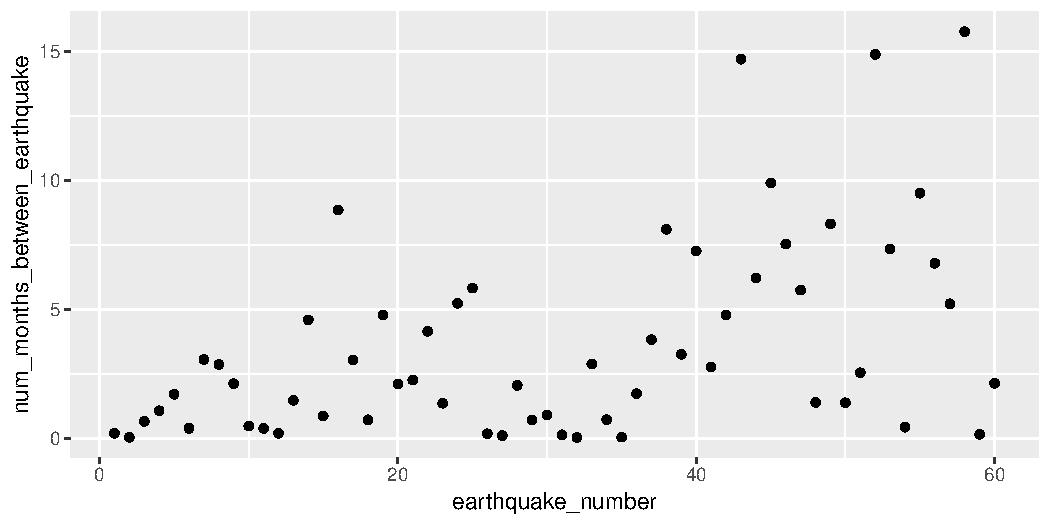
\includegraphics[width=4.5in]{earthquake_plot.pdf}
    \label{fig:enter-label}
\end{figure}

The time between earthquakes is known to be exponentially distributed. We suspect the distribution's mean changed once (at some point). So the DGP for the above data will be:

\beqn
X_1, X_2, \ldots, X_{\theta_3} \iid \theta_1 e^{-\theta_1 x} ~~\text{independent of}~~ X_{\theta_3 + 1}, X_{\theta_3 + 2}, \ldots, X_n \iid \theta_2 e^{-\theta_2 x}
\eeqn

\noindent For this problem, you may need to know some of these facts about the gamma distribution:

\beqn
Y \sim \text{Gamma}(\alpha, \beta) := \frac{\beta^\alpha}{\Gamma(\alpha)} y^{\alpha - 1} e^{-\beta y} \indic{y > 0}, ~~ F(y) = P(\alpha, \beta y),~~S(y) = Q(\alpha, \beta y)
\eeqn

\noindent where $P,Q$ are the lower and upper regularized gamma functions.

\begin{enumerate}[(a)]

\subquestionwithpoints{2} How many parameters can you draw inference for in this DGP?
%
\iftoggle{solutions}{\inred{
\beqn
3
\eeqn
}}{~\spc{0.5}}
%

\subquestionwithpoints{5} Find the likelihood of the data, $f(\x; \theta_1, \theta_2, \theta_3)$. Denote the sample size as $n$ i.e., do not use its known value of 60 here. You can assume all $x_i > 0$.
%
\iftoggle{solutions}{\inred{
\beqn
f(\x; \theta_1, \theta_2, \theta_3) &=& \prod_{i=1}^{\theta_3} f(x_i; \theta_1) \prod_{\theta_3 +1}^n f(x_i; \theta_2) \\
 &=& \prod_{i=1}^{\theta_3} \theta_1 e^{-\theta_1 x_i} \prod_{\theta_3 +1}^n \theta_2 e^{-\theta_2 x_i} \\
 &=& \theta_1^{\theta_3} e^{-\theta_1 \sum_{i=1}^{\theta_3} x_i} \theta_2^{n-\theta_3} e^{-\theta_2 \sum_{i=\theta_3 + 1}^{n} x_i}
\eeqn
}}{~\spc{5}}
%
\pagebreak

\subquestionwithpoints{3} Assume Laplace's prior of indifference. State the prior for all parameters below. Use correct unambiguous notation.
%
\iftoggle{solutions}{\inred{
\beqn
f(\theta_1, \theta_2, \theta_3) \propto 1
\eeqn
}}{~\spc{1}}
%


\subquestionwithpoints{3} The posterior is denoted $f(\theta_1, \theta_2, \theta_3~|~\x)$. Find its kernel.
%
\iftoggle{solutions}{\inred{
\beqn
f(\theta_1, \theta_2, \theta_3~|~\x) &\propto& f(\x; \theta_1, \theta_2, \theta_3) f(\theta_1, \theta_2, \theta_3) \\
&=& \parens{\theta_1^{\theta_3} e^{-\theta_1 \sum_{i=1}^{\theta_3} x_i} \theta_2^{n-\theta_3} e^{-\theta_2 \sum_{i=\theta_3 + 1}^{n} x_i}}(1) \\
&=& \theta_1^{\theta_3} e^{-\theta_1 \sum_{i=1}^{\theta_3} x_i} \theta_2^{n-\theta_3} e^{-\theta_2 \sum_{i=\theta_3 + 1}^{n} x_i}
\eeqn
}}{~\spc{5}}
%

\subquestionwithpoints{2} Circle one: this kernel is the kernel of a distribution which is ... \quad known \quad /  \quad \iftoggle{solutions}{\inred{unknown}}{unknown}

\subquestionwithpoints{4} We wish to create a Gibbs sampler now. Find the conditional distribution $f(\theta_1~|~\x, \theta_2, \theta_3)$ and give its brand name. Note that $\theta_1$ is a mean time and thus it's greater than 0.
%
\iftoggle{solutions}{\inred{
\beqn
f(\theta_1~|~\x, \theta_2, \theta_3) \propto \theta_1^{\theta_3} e^{-\theta_1 \sum_{i=1}^{\theta_3} x_i} \propto \text{Gamma}\parens{\theta_3 + 1, \sum_{i=1}^{\theta_3} x_i}
\eeqn
}}{~\spc{3.5}}
%

\subquestionwithpoints{4} Find the conditional distribution $f(\theta_2~|~\x, \theta_1, \theta_3)$ and give its brand name. Note that $\theta_2$ is a mean time and thus it's greater than 0.
%
\iftoggle{solutions}{\inred{
\beqn
f(\theta_2~|~\x, \theta_2, \theta_3) \propto \theta_2^{n-\theta_3} e^{-\theta_2 \sum_{i=\theta_3 + 1}^{n} x_i} \propto \text{Gamma}\parens{n - \theta_3 + 1, \sum_{i=\theta_3 + 1}^{n} x_i}
\eeqn
}}{~\spc{3.5}}
%
\pagebreak

\subquestionwithpoints{6} Find the conditional distribution $p(\theta_3~|~\x, \theta_1, \theta_2)$. Assume the parameter space of $\theta_3$ is $\braces{1,2, \ldots, n-1}$.
%
\iftoggle{solutions}{\inred{
\beqn
p(\theta_3~|~\x, \theta_1, \theta_2) &\propto& \theta_1^{\theta_3} e^{-\theta_1 \sum_{i=1}^{\theta_3} x_i} \theta_2^{-\theta_3} e^{-\theta_2 \sum_{i=\theta_3 + 1}^{n} x_i} \\
\text{Normalizing to sum to one,}~~ p(\theta_3~|~\x, \theta_1, \theta_2) &=& \frac{\theta_1^{\theta_3} e^{-\theta_1 \sum_{i=1}^{\theta_3} x_i} \theta_2^{-\theta_3} e^{-\theta_2 \sum_{i=\theta_3 + 1}^{n} x_i}}{\sum_{t=1}^{n-1} \theta_1^{t} e^{-\theta_1 \sum_{i=1}^{t} x_i} \theta_2^{-t} e^{-\theta_2 \sum_{i=t + 1}^{n} x_i}}
\eeqn
}}{~\spc{8}}


\subquestionwithpoints{3} Assume all conditional distributions are correct. We run the Gibbs Sampler for 10,000 runs and burn appropriately. Then we look at the autocorrelations for all chains (see next page). At what point should we thin if we wish to retain as many iterations as possible?
%
\iftoggle{solutions}{\inred{
\beqn
5
\eeqn
}}{~\spc{0.5}}
%


\subquestionwithpoints{3} After thinning, how many samples would be lift in the Gibbs chains approximately? (Assume we burned a very small number of iterations).
%
\iftoggle{solutions}{\inred{
\beqn
2000
\eeqn
}}{~\spc{0.5}}
%
\pagebreak

\begin{figure}[h]
    \centering
    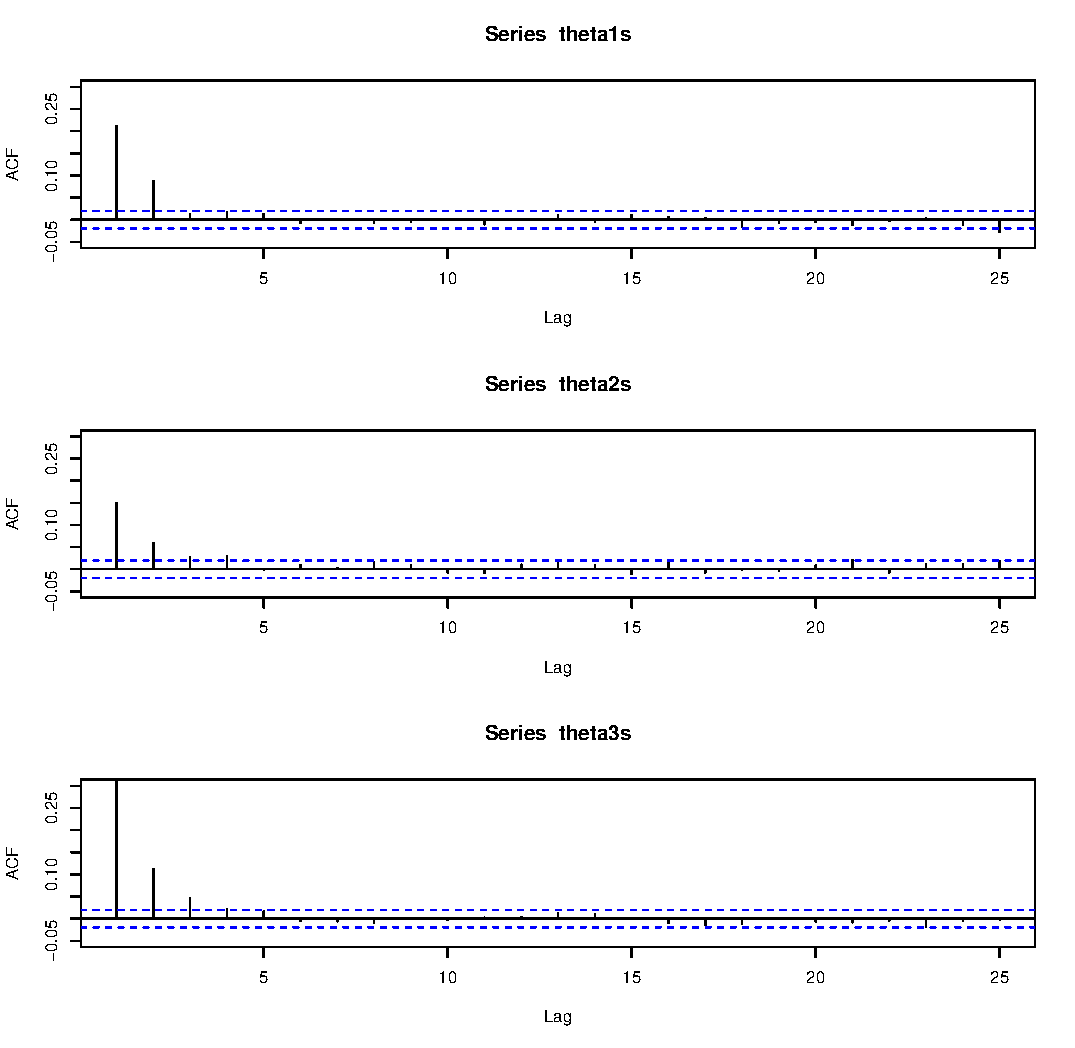
\includegraphics[width=7in]{autocorrelations.pdf}
    \label{fig:enter-label}
\end{figure}
\FloatBarrier




\subquestionwithpoints{3} Assume we thinned appropriately. Here is the histogram of the samples of $\theta_3$ given $\x$. What is your point estimate of $\theta_3$? Approximate it from the samples. No need to justify. 
%
\iftoggle{solutions}{\inred{
\beqn
29
\eeqn
}}{~\\~\\Your answer: }
%

\begin{figure}[h]
    \centering
    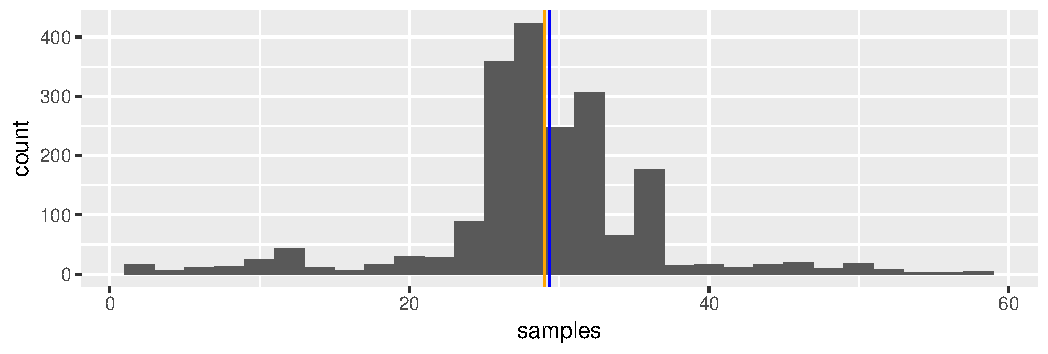
\includegraphics[width=5in]{theta3s.pdf}
    \label{fig:enter-label}
\end{figure}
\FloatBarrier

\subquestionwithpoints{4} Here is the histogram of the samples of $\theta_1$ given $\x$. Provide a 95\% CR for $\theta_1$. Approximate it from the samples. No need to justify. 
%
\iftoggle{solutions}{\inred{
\beqn
[0.3, 0.8]
\eeqn
}}{~\\~\\Your answer: }
%

\begin{figure}[h]
    \centering
    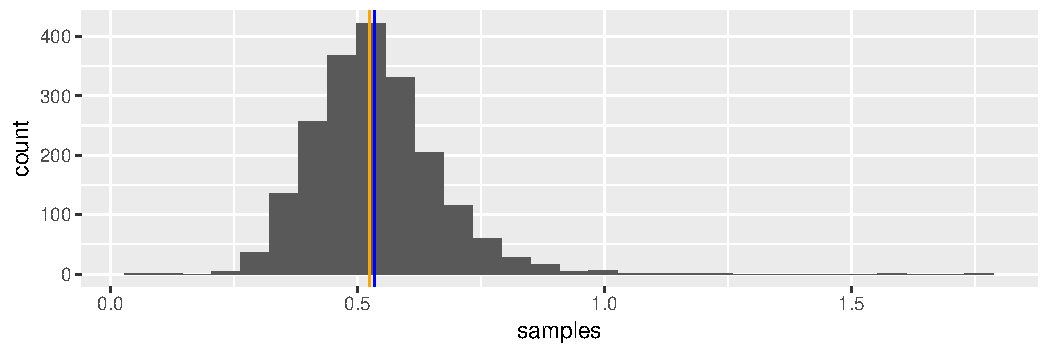
\includegraphics[width=5in]{theta1s.pdf}
    \label{fig:enter-label}
\end{figure}
\FloatBarrier

\subquestionwithpoints{4} Here is the histogram of the samples of $\theta_1$ given $\x$ minus the samples of $\theta_2$ given $\x$. Provide a decision on $H_0: \theta_1 = \theta_2$. No need to justify. 
%
\iftoggle{solutions}{\inred{
\beqn
\text{Reject $H_0$}
\eeqn

}}{~\\~\\Your answer: }
%

\begin{figure}[h]
    \centering
    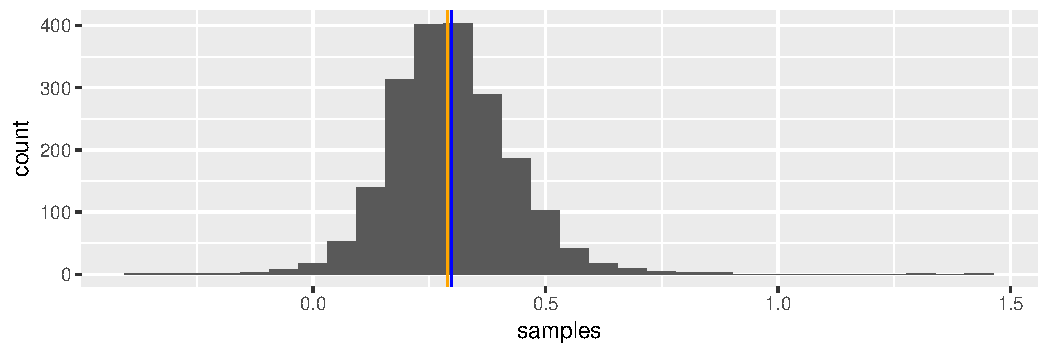
\includegraphics[width=5in]{diffs.pdf}
    \label{fig:enter-label}
\end{figure}
\FloatBarrier
\end{enumerate}
\pagebreak

\problem We collect data on yearly returns (in percentage) of two financial assets. The returns come from $DGP_1$ and $DGP_2$ respectively. The sample sizes are $n_1 = 17$ and $n_2 = 37$. Some statistics are as follows: $\xbar_1 = 6.17$, $s_1 = 1.91$, $\xbar_2 = 6.28$, $s_2 = 3.09$. 


\begin{enumerate}[(a)]

\subquestionwithpoints{2} We run a two-sample permutation test. What is the null hypothesis?
%
\iftoggle{solutions}{\inred{
\beqn
H_0: DGP_1 = DGP_2
\eeqn
}}{~\spc{1}}
%

\subquestionwithpoints{4} If we were to run all the permutation samples, how many samples would there be? You can answer using any well-known mathematical notation. You do not need to explicitly provide the number itself.
%
\iftoggle{solutions}{\inred{
\beqn
\binom{17+37}{17} = \binom{17+37}{37} = \binom{54}{17} = \binom{54}{37}
\eeqn
}}{~\spc{1.5}}


\subquestionwithpoints{4} We run a permutation test using $B = 10^5$ with the test statistic defined as $\xbar_1 - \xbar_2$. Below is a histogram of the samples. 


\begin{figure}[h]
    \centering
    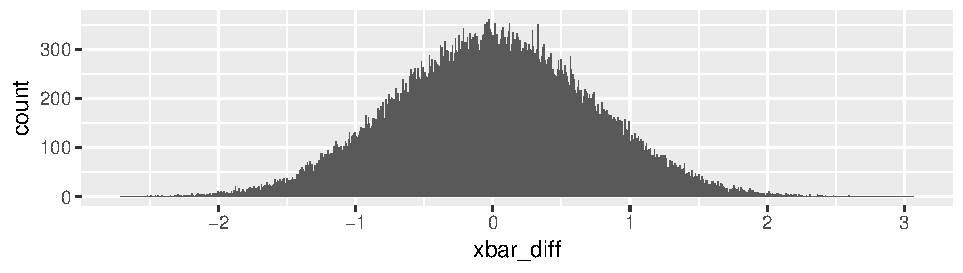
\includegraphics[width=6in]{xbar_diffs.pdf}
    \label{fig:enter-label}
\end{figure}
\FloatBarrier

Test the hypothesis in (a) at $\alpha = 5\%$. Justify why you retained or rejected. 
%
\iftoggle{solutions}{\inred{
~\\~\\ Retain $H_0$. The true test statistic from the raw data is $\xbar_1 - \xbar_2 = -0.11$ which falls within a 95\% RET which estimated above looks to be about $\bracks{-1.5,1.5}$.
}}{~\spc{6}}
\pagebreak


\subquestionwithpoints{4} We run a permutation test using $B = 10^5$ with the test statistic defined as $s_1 - s_2$. Below are some quantiles for all the $B$ test statistics:

\begin{verbatim}
> quantile(test_stats, c(0.025, 0.975))
     2.5%     97.5% 
-1.241878  1.264630    
\end{verbatim}

Test the hypothesis in (a) at $\alpha = 5\%$. Justify why you retained or rejected. 
%
\iftoggle{solutions}{\inred{
~\\~\\ 
Reject $H_0$. The true test statistic from the raw data is $s_1 - s_2 = -1.18$ which falls outside of the 95\% RET given above.
}}{~\spc{6}}

\subquestionwithpoints{2} Circle one: did you have to make any parametric assumptions to run the test in (d)? \quad yes \quad /  \quad \iftoggle{solutions}{\inred{no}}{no}

\subquestionwithpoints{2} The tests in both (c) and (d) share the same $H_0$. Circle one: do the tests in (c) and (d) share the same power? \quad yes \quad /  \quad \iftoggle{solutions}{\inred{no}}{no}

\end{enumerate}
\pagebreak

\problem We are interested in the differential survival (measured in days) of lung cancer patients by the amount of daily calories they consume in their diet. There are $n = 181$ total subjects in the study. Group 1 is those that consume more than 1200 per day (and there are $n_1 = 32$) and the number that consume 1000 calories or less per day is $n_2 = 149$. Below are the KM curves. The + signs indicate a censored observation.

\vspace{-0.55cm}
\begin{figure}[h]
    \centering
    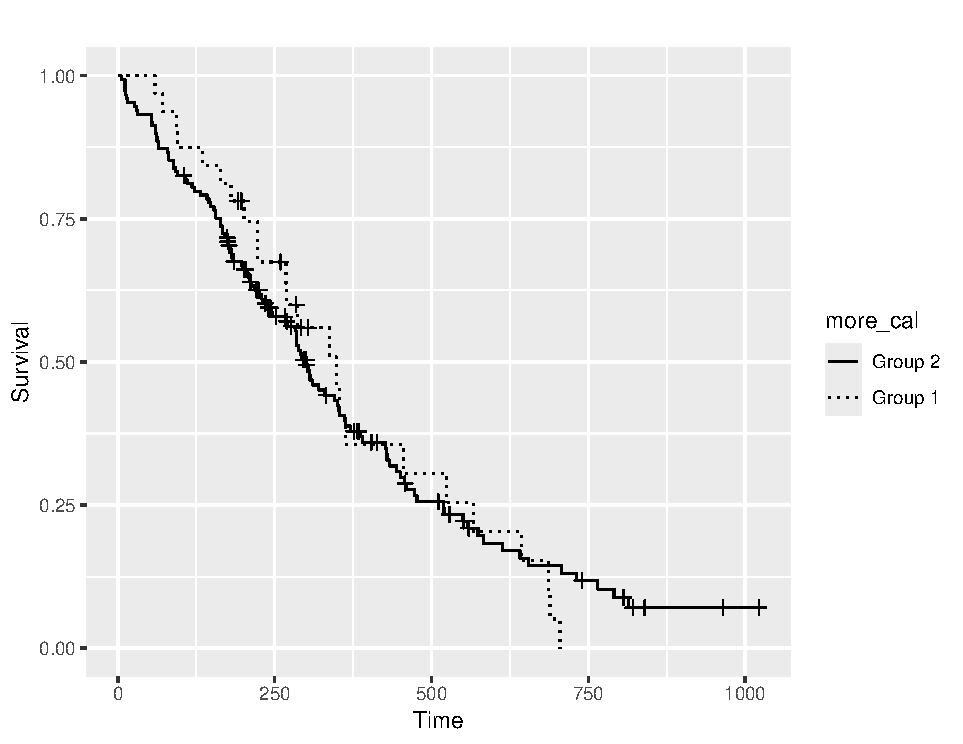
\includegraphics[width=6.0in]{kms.pdf}
    \label{fig:enter-label}
\end{figure}
\FloatBarrier

\begin{enumerate}[(a)]

\subquestionwithpoints{6} Assume for this question only there are \textit{no censored observations} (even though we know it's not true). Provide an approximate 95\% CI for survival more than 750 days in Group 2 (those that consume less than or equal to 1200 calories per day) to the nearest three digits.

%
\iftoggle{solutions}{\inred{
\beqn
CI_{S(y), 1-\alpha} &\approx& \bracks{\doublehat{S}(y) \pm z_{1- \overtwo{\alpha}} \sqrt{\frac{\doublehat{S}(y) (1 - \doublehat{S}(y))}{n}}~} \\
CI_{S(750), 95\%} &\approx& \bracks{0.12 \pm 1.96 \sqrt{\frac{0.12 (1 - 0.12)}{149}}~} = \bracks{0.068, 0.172}
\eeqn
}}{~\spc{5}}
\pagebreak

\subquestionwithpoints{2} Circle one: do the censored observations need to have the same observed survival times? \quad yes \quad /  \quad \iftoggle{solutions}{\inred{no}}{no}

\subquestionwithpoints{3} Circle one: the observation with the greatest value for group 2 is censored? \quad \iftoggle{solutions}{\inred{yes}}{yes} \quad /  \quad no

\subquestionwithpoints{4} Consider the following R code

\begin{verbatim}
#n_1: number of subjects in group 1
#n_2: number of subjects in group 2
#y_1: survival times for group 1
#y_2: survival times for group 2
#c_1: censor vector for group 1
#c_2: censor vector for group 2

B = 5000
median_diffs = array(NA, B)
for (b in 1 : B){
  idx_1_b = sample(1 : n_1, n_1, replace = TRUE) 
  idx_2_b = sample(1 : n_2, n_2, replace = TRUE) 
  y_1_b = y_1[idx_1_b]
  c_1_b = c_1[idx_1_b]
  y_2_b = y_2[idx_2_b]
  c_2_b = c_2[idx_2_b]
  km_1 = survfit2(Surv(y_1_b, c_1_b) ~ 1)
  km_2 = survfit2(Surv(y_2_b, c_2_b) ~ 1)
  res_1 = summary(km_1)$table
  res_2 = summary(km_2)$table
  median_diffs[b] = res_1["median"] - res_2["median"]
} 
\end{verbatim}

What is (1) the type of test used here and (2) the null hypothesis?
\iftoggle{solutions}{\inred{
\beqn
\text{(1) bootstrap (2) $H_0:$ the median survival in both groups are equal}
\eeqn
}}{~\spc{1}}
\pagebreak


\subquestionwithpoints{6} Below is a histogram of the $B$ values of \texttt{median\_diffs} from the previous R code. Run the test from the previous question at $\alpha = 5\%$ and justify the decision.

\begin{figure}[h]
    \centering
    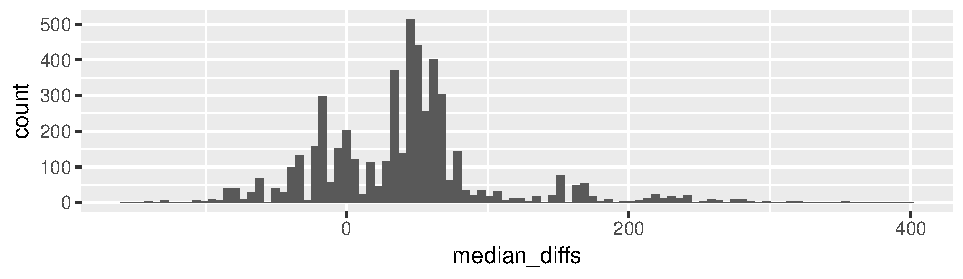
\includegraphics[width=6.5in]{median_diffs.pdf}
    \label{fig:enter-label}
\end{figure}
\FloatBarrier

\iftoggle{solutions}{\inred{
\beqn
\text{Retain $H_0$ since 0 is within the 95\% bootstrap CI for median differences.}
\eeqn
}}{~\spc{4}}

\subquestionwithpoints{5} We now wish to test $H_0$: the survival DGP for group 1 is the same as the survival DGP for group 2. We use the Log Rank test. Here is some relevant numeric output:

\begin{verbatim}
                   n Observed Expected (O-E)^2/E 
more_cal=Group 2 149      110    109.8  0.000274  
more_cal=Group 1  32       24     24.2  0.001243  
\end{verbatim}

Make a decision on $H_0$ at $\alpha = 5\%$.

\iftoggle{solutions}{\inred{
The log rank statistic is the sum of the $(O-E)^2/E$ column which is near zero, i.e. much less than the $\chisq{1}$ cutoff at $\alpha = 5\%$ which is $1.96^2 = 3.84$. Hence we retain $H_0$.
}}{~\spc{1}}
\pagebreak

\subquestionwithpoints{8} We now fit an iid Gamma model to group 2's survival data i.e. we assume the positive values $\y := <y_{2,1}, y_{2,2}, \ldots, y_{2,n_2}>$ were drawn from the DGP

\beqn
Y_{2,1}, Y_{2,2}, \ldots, Y_{2,n_2} \iid \text{Gamma}(\theta_1, \theta_2)
\eeqn

and we also have the censoring binary data $\bv{c} := <c_{2,1}, c_{2,2}, \ldots, c_{2,n_2}>$. Write the likelihood for the parameters. You may need to use the facts about the gamma distribution (see Problem 1). No need to simplify.

\iftoggle{solutions}{\inred{
\beqn
\mathcal{L}(\theta_1, \theta_2; \y, \bv{c}) &=& \prod_{\braces{i: c_i = 1}} f(y_i; \theta_1, \theta_2) \prod_{\braces{i: c_i = 0}} S(y_i) \\
&=& \prod_{\braces{i: c_i = 1}} \frac{\theta_2^{\theta_1}}{\Gamma(\theta_1)} y_i^{\theta_1 - 1} e^{-\theta_2 y_i} \prod_{\braces{i: c_i = 0}} Q(\theta_1, \theta_2 y_i) \\
%&=& \frac{\theta_2^{m \theta_1}}{\Gamma(\theta_1)^m} \parens{\prod_{\braces{i: c_i = 1}} y_i}^{\theta_1 - 1} e^{-\theta_2 \sum_{\braces{i: c_i = 1}}  y_i} \prod_{\braces{i: c_i = 0}} Q(\theta_1, \theta_2 y_i) 
\eeqn
}}{~\spc{12}}


\subquestionwithpoints{2} Circle one: does the likelihood in the previous question have a closed form solution for either parameter? \quad yes \quad /  \quad \iftoggle{solutions}{\inred{no}}{no}

\end{enumerate}

\end{document}



\problem Benford's Law represents the distribution of the leading digit in base-10 numbers within datasets across a wide variety of natural phenomenon such as street addresses, stock prices, population numbers, etc:

\beqn
X \sim \text{Benford} := \logbaseten{\frac{x+1}{x}} \indic{x \in \braces{1, 2, \ldots, 9}}, \quad \theta_0 := \expe{X} = 3.44, \quad \sigsq_0 := \var{X} = 6.06
\eeqn

\noindent For example, here are 15 numbers sampled from Benford's Law sorted: 1\ingray{1217} 1\ingray{1426} 1\ingray{2612} 1\ingray{3368} 1\ingray{5644} 2\ingray{5311} 2\ingray{7342} 3\ingray{9332} 4\ingray{1511} 4\ingray{2632} 4\ingray{4125} 5\ingray{2322} 7\ingray{8431} 8\ingray{1673} 8\ingray{2152}. Notice how the first digit (in black) is more likely to be a 1 or 2 vs an 8 or 9.


Let the parameter of interest be the mean value of the first digit of numeric entries (call it $\theta$). Benford's Law is used by the Internal Revenue Service (IRS) to catch people committing tax fraud since numeric entries on tax forms is known to follow Benford's law. 



 


\begin{enumerate}[(a)]

\subquestionwithpoints{2} Circle one: the value of $\theta$, then mean numeric value of the first digit for the fields in any individual's tax return is... \quad known \quad /  \quad \iftoggle{solutions}{\inred{unknown}}{unknown}

\subquestionwithpoints{2} To catch someone cheating on their taxes, we need to prove beyond a reasonable doubt that this individual's $\theta$ is not the expectation value of Benford's Law. Thus the alternative hypothesis is $H_a: \theta \neq 3.44$. What is the null hypothesis for the parameter $\theta$?
%
\iftoggle{solutions}{\inred{
\beqn
H_0: \theta = 3.44
\eeqn
}}{~\spc{0}}
%
\subquestionwithpoints{2} The \qu{1040 form} the IRS uses has 52 numeric entries. We collect the first digit from each of these fields. Let these digits be the data $x_1, x_2, \ldots, x_{52}$. What is the value of $n$?
\iftoggle{solutions}{\inred{
$n = 52$
}}{~\spc{0}}
%
\subquestionwithpoints{2} What estimator would you choose to estimate $\theta$? $\thetahat = $ \iftoggle{solutions}{\inred{
$\Xbar$
}}{~\spc{0}}
%
\subquestionwithpoints{2} Regardless of what answer you put for the previous question, for the remainder of this problem use $\thetahat = \Xbar$. Circle one: the distribution of this estimator is... \quad known exactly \quad /  \quad \iftoggle{solutions}{\inred{unknown}}{unknown}


\subquestionwithpoints{5}  Compute $RET_{5\%}$, the retainment region at $\alpha = 5\%$. Remember, the full null hypothesis is that the data DGP is $\Xoneton \iid$ Benford. Round the values to the nearest two decimals.

\iftoggle{solutions}{\inred{
\beqn
\text{RET}_{5\%} = \bracks{\theta_0 \pm z_{1-\frac{\alpha}{2}} \frac{\sigma_0}{\sqrt{n}}} = \bracks{3.44 \pm 1.96 \frac{\sqrt{6.06}}{\sqrt{52}}} = \bracks{3.44 \pm 0.67} = \bracks{2.77, 4.11}
\eeqn\pagebreak
}}{~\spc{6}}


\subquestionwithpoints{2} Circle one: the RET above is... \quad exact \quad /  \quad \iftoggle{solutions}{\inred{approximate}}{approximate}

\subquestionwithpoints{6} For Bob's tax return, $\xbar = 5.27$ for the 52 first digits of the numeric fields. Run the test and write a concluding sentence.
%

\iftoggle{solutions}{\inred{
$\xbar \notin \text{RET}_{5\%}$ hence we reject $H_0$ and conclude that there is statistically significant evidence that the first digits of  Bob's numeric values on his form 1040 do not adhere to Benford's Law, i.e., Bob is cheating the IRS.
}}{~\spc{5}}



\subquestionwithpoints{3} Circle one: you could've made a ... \quad \iftoggle{solutions}{\inred{Type I error}}{Type I error} \quad /  \quad Type II error 

\subquestionwithpoints{6} Fisher's approximate $p_{val}$ for this test equals $2\prob{Z > z}$ where $Z \sim \stdnormnot$. Compute the value of $z$ to the nearest two decimals.
%
\iftoggle{solutions}{\inred{
\beqn
p_{val} &=& 2 \cprob{\thetahat > \thetahathat}{H_0} = 2\cprob{\Xbar > \xbar}{H_0} = 2 \prob{\frac{\Xbar - \theta_0}{\sigma_0 / \sqrt{n}} > \frac{\xbar - \theta_0}{\sigma_0 / \sqrt{n}}} \\
&=& 2\prob{Z > \frac{5.27 - 3.44}{\sqrt{6.06} / \sqrt{52}}} \mathimplies  z = 5.36
\eeqn
}}{~\spc{5}}


\subquestionwithpoints{6} Compute an approximate $CI_{\theta, 95\%}$ to the nearest two decimals.
%

\iftoggle{solutions}{\inred{
\beqn
CI_{\theta, 95\%} = \bracks{\xbar \pm z_{1-\frac{\alpha}{2}} \frac{\sigma_0}{\sqrt{n}}} = \bracks{5.27 \pm 1.96 \frac{\sqrt{6.06}}{\sqrt{n}}} = \bracks{5.27 \pm 0.67} = \bracks{4.60, 5.94}
\eeqn\pagebreak
}}{~\spc{6}}

\subquestionwithpoints{8} When people commit fraud, they may fabricate numbers \qu{completely randomly}. This means the first digits of their numbers are drawn from the DGP:

\beqn
\Xoneton \iid U(\braces{1,2, \ldots, 9})~~\text{where}~~ \theta := \expe{X} = 5, \quad \sigsq := \var{X} = 6.67
\eeqn

How many digits $n$ would you need to detect if someone was cheating by sampling numbers randomly (via the above DGP) with probability 90\% if the null assumption is the same as previously, i.e. the DGP is $\Xoneton \iid$ Benford. Note that $z_{10\%} = -1.28$. Assume $\alpha = 5\%$. Round the result to the nearest natural number.

\iftoggle{solutions}{\inred{
% From part (f), we know that

% \beqn
% \text{RET}_{5\%} = \bracks{\theta_0 \pm z_{1-\frac{\alpha}{2}} \frac{\sigma}{\sqrt{n}}} = \bracks{3.44 \pm 1.96 \frac{\sqrt{6.06}}{\sqrt{n}}} = \bracks{3.44 - \frac{4.825}{\sqrt{n}}, 3.44 + \frac{4.825}{\sqrt{n}}}
% \eeqn

As the \qu{real} $\thetahat$ distribution is centered to the right of the $\thetahat~|~H_0$ distribution, we must equate the right bound of the retainment region (from part f) to the 10\%ile of the distribution of $\thetahat$ and solve for the sample size $n$:

\beqn
\theta_0 + z_{1-\frac{\alpha}{2}} \frac{\sigma_0}{\sqrt{n}} &=& \theta + z_{10\%} \frac{\sigma}{\sqrt{n}} \\
3.44 + 1.96 \frac{\sqrt{6.06}}{\sqrt{n}} &=& 5 - 1.28 \frac{\sqrt{6.67}}{\sqrt{n}} \\
1.96 \frac{\sqrt{6.06}}{\sqrt{n}} + 1.28 \frac{\sqrt{6.67}}{\sqrt{n}} &=& 1.56 \\
\frac{8.13}{\sqrt{n}} &=& 1.56 \\
n &=& \squared{\frac{8.13}{1.56}} = 27.165 \mathimplies n=27
\eeqn

}}{~\spc{9}}



\end{enumerate}


\problem Consider the \qu{inverse gamma} DGP, a famous rv we'll study later in class:

\beqn
\Xoneton \sim \text{InvGamma}(\theta_1, \theta_2) := \frac{\theta_2^{\theta_1}} {\Gamma(\theta_1)} x^{-\theta_1 - 1} e^{-\theta_2 / x} \indic{x>0}
\eeqn

\noindent where $\Gamma(u)$ is called the \qu{gamma} function which is $\reals \rightarrow \reals$ and ensures the Humpty-Dumpty identity. The mean and variance of this rv are given below:

\beqn
\expe{X} = \frac{\theta_2}{\theta_1 - 1}, ~~ \var{X} = \frac{\theta_2^2}{(\theta_1 - 1)^2 (\theta_1 - 2)}
\eeqn

\begin{enumerate}[(a)]

\subquestionwithpoints{2} How many parameters can be targets of inference in this DGP? \iftoggle{solutions}{\inred{2}\pagebreak}{~\spc{1}}


% \subquestionwithpoints{3} What is a method of moments estimator for $\var{X}$? Your answer must use notation known from class or be a function of $\Xoneton$, $n$ and fundamental constants only. 
% %
% \iftoggle{solutions}{\inred{
% \beqn
% \hat{\sigma}^2_n := \oneover{n} \sum_{i=1}^n (X_i - \Xbar)^2
% \eeqn\pagebreak
% }}{~\spc{3}}

\subquestionwithpoints{8} Show that the method moments estimator for $\theta_1$ is $\hat{\theta}_1^{MM} = \frac{2\muhat_2 -\muhat_1^2}{\muhat_2 - \muhat_1^2}$.
%
\iftoggle{solutions}{\inred{
\beqn
\mu_1 &:=& \expe{X} = \frac{\theta_2}{\theta_1 - 1} \mathimplies \theta_2 = \mu_1 (\theta_1 - 1) \\
\mu_2 - \mu_1^2 &:=& \expe{X^2} - \expe{X}^2 = \var{X} = \frac{\theta_2^2}{(\theta_1 - 1)^2 (\theta_1 - 2)} \\
&=& \frac{(\mu_1 (\theta_1 - 1))^2}{(\theta_1 - 1)^2 (\theta_1 - 2)} \\
&=& \frac{\mu_1^2}{\theta_1 - 2} \\
\mathimplies \theta_1 - 2 &=& \frac{\mu_1^2}{\mu_2 - \mu_1^2} \\
\mathimplies \theta_1 &=& \frac{\mu_1^2}{\mu_2 - \mu_1^2} + 2 = \frac{\mu_1^2}{\mu_2 - \mu_1^2} + 2 \frac{\mu_2 - \mu_1^2}{\mu_2 - \mu_1^2} \mathimplies \hat{\theta}_1^{MM} = \frac{2\muhat_2 -\muhat_1^2}{\muhat_2 - \muhat_1^2}
\eeqn

That completes the problem. But we'll need $\hat{\theta}_2^{MM}$ for the next problem, so we'll derive it here now by substituting $\hat{\theta}_1^{MM}$ for $\theta_1$:

\beqn
\theta_2 &=& \mu_1 (\theta_1 - 1) \\
&=& \mu_1 \parens{\frac{2\mu_2 -\mu_1^2}{\mu_2 - \mu_1^2} - 1} = \mu_1 \parens{\frac{2\mu_2 -\mu_1^2}{\mu_2 - \mu_1^2} - \frac{\mu_2 - \mu_1^2} {\mu_2 - \mu_1^2}} \\
\mathimplies \hat{\theta}_2^{MM} &=& \frac{\muhat_1\muhat_2}{\muhat_2 - \muhat_1^2}
\eeqn
}}{~\spc{12}}


\subquestionwithpoints{2} Circle one: as $n$ gets larger, the $\mse{\hat{\theta}_2^{MM}}$ ... \iftoggle{solutions}{\inred{decreases}}{decreases}\quad / \quad increases

\subquestionwithpoints{3} Let $\x = <0.918, 0.386, 0.395, 0.553, 1.643, 0.536>$. Using the method of moments estimation technique, find the estimates for the two parameters $\doublehat{\theta}_1^{MM}$ and $\doublehat{\theta}_2^{MM}$. Round to three decimals.

\iftoggle{solutions}{\inred{
We first estimate the moments and then substitute

\beqn
\muhathat_1 = \oneover{n} \sum_{i=1}^n x_i = 0.7385, \quad\quad \muhathat_2 = \oneover{n} \sum_{i=1}^n x_i^2 = 0.7400 \\
\doublehat{\theta}_1^{MM} = \frac{2\muhathat_2 -\muhathat_1^2}{\muhathat_2 - \muhathat_1^2} = 4.802, \quad\quad 
\doublehat{\theta}_2^{MM} = \frac{\muhathat_1\muhathat_2}{\muhathat_2 - \muhathat_1^2} = 2.807
\eeqn\pagebreak
}}{~\spc{9}}



\subquestionwithpoints{8} Assume we now know that $\theta_1 = 5$ going forward in this problem. Show that the maximum likelihood estimator for the second parameter for $n$ draws from this inverse gamma DGP is $\thetahatmle_2 = 5n \inverse{\sum_{i=1}^n X_i^{-1}}$.

\iftoggle{solutions}{\inred{
\beqn
\mathcal{L} &=& \prod_{i=1}^n \frac{\theta_2^{5}} {\Gamma(5)} X_i^{-5 - 1} e^{-\theta_2 / X_i} = \frac{\theta_2^{5n}} {\Gamma(5)^n} e^{-\theta_2 \sum_{i=1}^n \oneover{X_i}} \prod_{i=1}^n X_i^{-6} \\
\ell &=& 5n \natlog{\theta_2} - n \natlog{\Gamma(5)}-\theta_2 \sum_{i=1}^n \oneover{X_i} + \natlog{\prod_{i=1}^n X_i^{-6}} \\
\ell' &=& \frac{5n}{\theta_2} - \sum_{i=1}^n \oneover{X_i} ~~{\buildrel set \over =}~~ 0 \mathimplies \frac{5n}{\theta_2} = \sum_{i=1}^n \oneover{X_i} \mathimplies \thetahatmle_2 = \frac{5n}{\displaystyle\sum_{i=1}^n X_i^{-1}}
\eeqn
}}{~\spc{12}}

% \subquestionwithpoints{3} Assume the dataset from part (d). Using the maximum likelihood estimation technique, find the estimate for the second parameter, $\thetahathatmle_2$. Round to three decimals.

% \iftoggle{solutions}{\inred{
% \beqn
% \thetahathatmle_2 &=& \frac{5n}{\displaystyle\sum_{i=1}^n x_i^{-1}} = \frac{5(6)}{\oneover{0.918} + \ldots + \oneover{0.536}} = 2.859
% \eeqn
% }}{~\spc{5}}

% \subquestionwithpoints{3} Provide two reasons \text{in English} why $\thetahathatmle_2$ will likely be more accurate than $\doublehat{\theta}_2^{MM}$.


% \iftoggle{solutions}{\inred{
% \begin{enumerate}[1.]
%     \item When computing $\thetahathatmle_2$ we assumed a value of $\theta_1$ which was not assumed when computing $\doublehat{\theta}_2^{MM}$.
%     \item Maximum likelihood estimators generally have smaller error than method of moments estimators.
% \end{enumerate}
% }}{~\spc{3}}


\subquestionwithpoints{6} Find the Cramer-Rao Lower Bound for any unbiased estimator for $\theta_2$.

\iftoggle{solutions}{\inred{
Using the log likelihood $\ell'$ from (e), we continue:

\beqn
\ell'' &=& -\frac{5n}{\theta_2^2} \\
I(\theta_2) &=& \expe{-\ell''} = \expe{-\parens{-\frac{5n}{\theta_2^2}}} = \frac{5n}{\theta_2^2} \\
\var{\thetahat_2} &\geq& \overn{I(\theta_2)^{-1}} = \frac{\inverse{\frac{5n}{\theta_2^2}}}{n} = \frac{\theta_2^2}{25n^2}
\eeqn\pagebreak
}}{~\spc{12}}

\end{enumerate}

\problem We are trying to prove that less than 2\% of all electronic devices a certain company manufactures are defective. Let $\theta$ denote the real proportion of defective devices.



\begin{enumerate}[(a)]

\subquestionwithpoints{2} What is the null hypothesis? \iftoggle{solutions}{\inred{$H_0: \theta \geq 0.02$}}{~\spc{0}}

\subquestionwithpoints{2} We now sample and record if the device is defective or not. What sampling procedure should be employed to ensure the results can be believed for the entire manufacturing process? \iftoggle{solutions}{\inred{simple random sample (SRS)}}{~\spc{0.5}}

\subquestionwithpoints{3} We sample $n=300$ according to the procedure given by the correct answer for (b). What is the DGP this sample was realized from?
%
\iftoggle{solutions}{\inred{
\beqn
\Xoneton \iid \bernoulli{\theta}
\eeqn
}}{~\spc{1}}


\subquestionwithpoints{5} We choose to use the binomial exact test. Below is a table of the PDF of the $\binomial{300}{0.02}$ rv.

\begin{table}[ht]
\centering
\begin{tabular}{r|rrrrrrrrrrr}
  \hline
 $x$ & 0 & 1 & 2 & 3 & 4 & 5 & 6 & 7 & 8 & 9 & 10 \\ 
  \hline 
  $p(x)$ & 0.002 & 0.014 & 0.044 & 0.088 & 0.134 & 0.162 & 0.162 & 0.139 & 0.104 & 0.069 & 0.041
\end{tabular}
\end{table}~\spc{-0.5}

Find the three smallest possible nonzero sizes of the binomial exact test each to the nearest three digits.

\iftoggle{solutions}{\inred{
The three possible sizes are the three left tails which are the CDF values $F(0), F(1), F(2)$ which are $0.002, 0.016, 0.060$.
}}{~\spc{2}}


\subquestionwithpoints{5}  Find $RET_{5\%}$, the retainment region at $\alpha = 5\%$. 

\iftoggle{solutions}{\inred{
Since $\alpha=5\%$, we cannot use $\braces{2,3, \ldots, 100}$ as this would result in a size of 6\%. Thus, we must use $\braces{1, 2, 3, \ldots, 100}$ resulting in a size of 1.6\% as it's the largest size $\leq \alpha$.\pagebreak
}}{~\spc{6}}

\subquestionwithpoints{5}  Of the 300 sampled devices, 3 were defective. Run the test. No need to write a concluding sentence.

\iftoggle{solutions}{\inred{
Since $3 \in RET_{5\%}$, we retain $H_0$.
}}{~\spc{3}}
 
\subquestionwithpoints{3} If you don't believe the result of this test but you believe the sampling was done correctly, what is a legitimate criticism of the experiment? \iftoggle{solutions}{\inred{The sample size was insufficiently large, i.e., the test was underpowered.}}{~\spc{2}}


\end{enumerate}
\end{document}


%%%%clinical significance!

